\chapter{Perulangan (\textit{Looping})}

\section{Perulangan}
Seperti sudah dijelaskan Bab Pengenalan Algoritma, perulangan(looping) merupakan salah satu stuktur dasar algoritma. Pada algoritma, perulangan dipanggil dengan menggunakan pernyataan (\textit{for}) dan (\textit{while}). Masing - masing dari pernyataan ini memiliki cara kerjanya masing - masing sesuai yang telah dijelaskan pada beberapa sub-bab sebelumnya. Bermodalkan kedua pernyataan perulangan, mari kita telusuri kapan sebenarnya struktur dasar algoritma perulangan digunakan.  \\

Struktur perulangan secara umum terdiri atas dua bagian : 
\begin{enumerate}
	\item \textbf{Kondisi Perulangan}, yaitu ekspresi boolean yang harus dipenuhi untuk melaksanakan perulangan. Kondisi ini ada yang dinyatakan secara eksplisit maupun implisit
		\item \textbf{Badan Perulangan(body)}, yaitu bagian algoritma yang akan diulang ketika kondisi dipenuhi
\end{enumerate}

Disamping itu, struktur pengulangan biasanya disertai dengan bagian berikut: 
\begin{enumerate}
	\item \textbf{inisialisasi}, yaitu aksi yang dilakukan sebelum pengulangan dilakukan pertama kali 
	\item \textbf{terminasi}, yaitu aksi yang dilakukan setelah pengulangan selesai dilaksanakan
\end{enumerate}
Inisialisasi dan terminasi tidak selalu arus ada, namun pada beberapa kasus (jika menggunakan \textit{while}), inisialiasi diperlukan

Bedasarkan peraturan diatas, struktur perulangan secara umum adalah sebagai berikut : 
\begin{Petunjuk}
\label{Ptk:Struktur Perulangan}
	\textbf{Struktur Perulangan}\\
		\textit{inisialiasi}\\
		\textit{awal pengulangan}(dengan / atau tanpa kondisi)\\
		~~~~~\textit{badan pengulangan}\\
		\textit{akhir pengulangan}\\
		\textit{terminasi}\\
\end{Petunjuk}

%Pernyataan \textit{for} digunakan untuk mengiterasi sebuah \textit{array}, \textit{list} ataupun kumpulan variabel/objek lainnya sedangkan pernyataan \textit{while} digunakan untuk perulangan yang berdasarkan kondisi tertentu.

\newpage

\subsection{Perulangan dengan \textit{for}}
Konstruksi \textit{for} digunakan untuk menghasilkan pengulangan sejumlah kali yang telah diberitahukan sebelumnya. Jumlah pengulangan sudah diketahui atau dapat ditentukan sebelum eksekusi. Perulangan \textit{for} juga bisa ditentukan dimulai dari kapan, berhenti pada saat kapan, dan melangkah seberapa banyak dari mulai sampai akhir. \\

Untuk struktur \textit{while} bisa dilihat sebagai berikut : 
\begin{tabbing}
\textbf{for} $i$ \textbf{in} $x$:~~~~~~~~~~~~~~~\=\#$x$ adalah \textit{kumpulan variabel}, iterasi dilakukan sebanyak panjang $x$\\
~~~~~statements\\
\end{tabbing}
\textbf{atau}
\begin{tabbing}
\textbf{for} $i$ \textbf{in} range([start=0],stop,[step=1]):\\
~~~~~badan pengulangan\\
\end{tabbing}


Contoh penggunaan format Python untuk iterasi isi dari List bisa dilihat di Listing \ref{lst:iterasiArray}.
\begin{listprog}{iterasiList.py}
	\label{lst:iterasiArray}
	\begin{lstlisting}[language=Python]
		A = [4,1,3,5]
		for i in A:
			print i
		#Hasil print berupa 4 1 3 5
	\end{lstlisting}
\end{listprog}

Sedangkan untuk mencetak rangkaian bilangan misalnya dari 1 sampai 10 bisa menggunakan fungsi \textit{range}. Contohnya bisa dilihat di Listing \ref{lst:cetakBilangan}
\begin{listprog}{cetakBilangan.py}
	\label{lst:cetakBilangan}
	\begin{lstlisting}[language=Python]
		for i in range(1,11):
			print i
		#Hasil print berupa 1 2 3 4 5 6 7 8 9 10
	\end{lstlisting}
\end{listprog}

\newpage

Untuk \textit{flowchart} \textit{for} bisa dilihat di Gambar \ref{fig:flowchartFor}.
\begin{figure}[h!]%
\centering
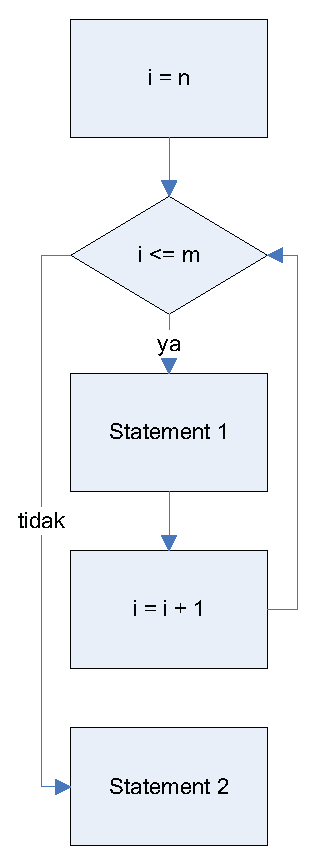
\includegraphics[scale=0.6]{fig/flowchart-FOR.eps}%
\caption{Flowchart For}%
\label{fig:flowchartFor}%
\end{figure}


\subsection{Perulangan dengan \textit{while}}
Konstruksi \textit{while} digunakan untuk menghasilkan pengulangan sejumlah kali selama kondisi ekspresi memenuhi. Badan perulangan pada \textit{while} akan dilaksanakan terus-menerus selama kondisi bernilai \textit{TRUE}. Jika kondisi sudah bernilai \textit{FALSE} maka badan perulangan tidak akan dimasuki dan pengulangan akan selesai.

\FloatBarrier
Untuk struktur \textit{while} bisa dilihat sebagai berikut.
\begin{tabbing}
\textbf{while} (Kondisi Logika):~~~~~~~~~~~~~~~\=\#Menjalankan perulangan selama kondisi benar\\
~~~~~statements\\
\end{tabbing}

Contoh penggunaan \textit{while} dalam bahasa Python untuk mencetak menurun bilang 10 sampai 1 bisa dilihat di Listing \ref{lst:cetakBilanganTurun}.
\begin{listprog}{cetakBilanganTurun.py}
	\label{lst:cetakBilanganTurun}
	\begin{lstlisting}[language=Python]
		i = 10
		while(i>0):
			print i
			i = i - 1	\end
		#Hasil print berupa 10 9 8 7 6 5 4 3 2 1
	\end{lstlisting}
\end{listprog}

\newpage
Untuk \textit{flowchart} \textit{while} bisa dilihat di Gambar \ref{fig:flowchartWhile}.
\begin{figure}[h!]%
\centering
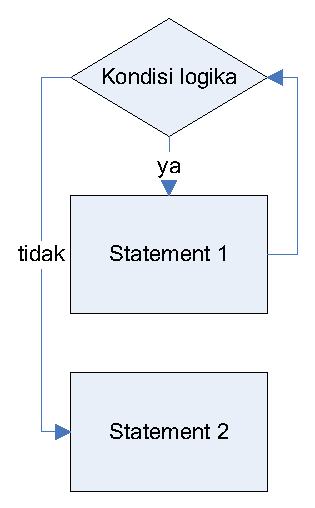
\includegraphics[scale=0.6]{fig/flowchart-WHILE.eps}%
\caption{Flowchart While}%
\label{fig:flowchartWhile}%
\end{figure}


\section{Implementasi Perulangan}
Pada sub-bab ini kita akan melihat bagaimana skenario - skenario penggunaan struktur pengulangan pada algoritma. Perulangan merupakan struktur dasar yang butuh waktu unuk dimengerti.Untuk mahir dalam pengulangan diperlukan banyak latihan dalam berbagai permasalahan yang melibatkan struktur perulangan.

Berikut ini adalah skenario - skenario dimana perulangan dibutuhkan : 
\begin{enumerate}
	\item Perulangan dibutuhkan bilamana kita ingin mengeksekusi perintah yang sama berkali-kali. Bayangkan pada keadaan dimana kita memerlukan pencetakan sebuah string sebanyak 10(Sepuluh) kali. Melakukan perintah sebanyak 10(Sepuluh) kali masih dapat di-manage dengan sequence(runtunan), tetapi bagaimana jika diminta 100.000(Seratus Ribu) kali. Tentunya ukuran kode sumber untuk algoritma akan membengkak seiring dengan jumlah perintah yang dilakukan. Perhatikan dua contoh berikut :
	
\begin{contoh}
	\label{cth:sequenceCetak}
	\textbf{Cetak Hello World Sepuluh Kali}
\begin{listprog}{SepuluhHello.py}
\label{lst:SepuluhHello}
\begin{lstlisting}[language=Python]
	print(``Hello, World!``)
	print(``Hello, World!``)
	print(``Hello, World!``)
	print(``Hello, World!``)
	print(``Hello, World!``)
	print(``Hello, World!``)
	print(``Hello, World!``)
	print(``Hello, World!``)
	print(``Hello, World!``)
	print(``Hello, World!``)
\end{lstlisting}
\end{listprog}
\end{contoh}

\begin{contoh}
	\label{cth:PengulanganCetak}
	\textbf{Perulangan Hello World}
\begin{listprog}{SepuluhHelloLoop.py}
\label{lst:SepuluhHelloLoop}
\begin{lstlisting}[language=Python]
	for i in range(10):
		print(``Hello, World!``)
\end{lstlisting}
\end{listprog}
\end{contoh}

Dari contoh \ref{cth:sequenceCetak} dan \ref{cth:PengulanganCetak} diatas, Anda dapat mengevaluasi sendiri jika \textit{Hello World} akan dicetak sebanyak 100.000 kali. Manakah yang lebih efisien menurut Anda ? \\ 
Pada kasus pembuatan algoritma pada dunia nyata, perulangan tidak hanya dipakai untuk melakukan eksekusi satu perintah saja namun lebih dari satu perintah yang sama berulang - ulang. Perhatikan contoh berikut :

\begin{contoh}
	\label{cth:PengulanganPerintahWhile}
	\textbf{Perulangan perintah jamak (\textit{while})}
\begin{listprog}{PerintahJamakWhile.py}
\label{lst:PerintahJamakWhile}
\begin{lstlisting}[language=Python]
	i = 1
	negasi = -1
	jumlah = 0
	while(i<=5):
		negasi = -negasi
		nilai = negasi * i 
		
		#sama dengan jumlah = jumlah + nilai
		jumlah += nilai	 
				
		print(nilai)
		i += 1 #lihat petunjuk sebelumnya
	print(jumlah)
\end{lstlisting}
\end{listprog}
	\end{contoh}

Perhatikan bahwa ada kondisi-kondisi yang mempengaruhi kapan statement perulangan  \textit{while} atau \textit{for} digunakan. Namun,  Perulangan \textit{while} atau \textit{for} dapat dikonversi menjadi struktur yang berbeda satu sama lain. Kita dapat melakukan konversi atas Contoh \ref{cth:PengulanganPerintahWhile} menjadi dalam bentuk perulangan  \textit{for} berikut : 

\begin{contoh}
	\label{cth:PengulanganPerintahFor}
	\textbf{Pengulangan perintah jamak (\textit{for})}
\begin{listprog}{PerintahJamakFor.py}
\label{lst:PerintahJamakFor}
\begin{lstlisting}[language=Python]
	negasi = -1
	jumlah = 0
	for i in range(5):
		negasi = -negasi
		nilai = negasi * (i+1) 
		jumlah += nilai					
		print(nilai)
	print(jumlah)
\end{lstlisting}
\end{listprog}
\end{contoh}

	\item Perulangan sering digunakan pada pemrosesan terhadap tipe-data jamak, misalnya \textit{array}, \textit{list}, \textit{string} dan bentuk tipe-data jamak lainnya yang membutuhkan penelusuran terhadap isi data yang lebih dari satu. Seluruh tipe-data jamak pada algoritma memiliki cara pemrosesan(baca/tulis) yang sama. Baik array, list, string atau tipe-data jamak lain semuanya memiliki properti indeks untuk mengakses data mana yang akan diproses.   
	
\FloatBarrier
\subsection{Array}
Array\sidenote{Di bahasa pemrograman Python, implementasi dari Array disebut sebagai List.} merupakan kumpulan dari variabel. Satu array bisa menampung beberapa data. Gambar \ref{fig:illustrasiArray} menunjukkan illustrasi dari sebuah array yang berkapasitas $j$. 
\begin{center}
	\begin{figure}[h!]%
		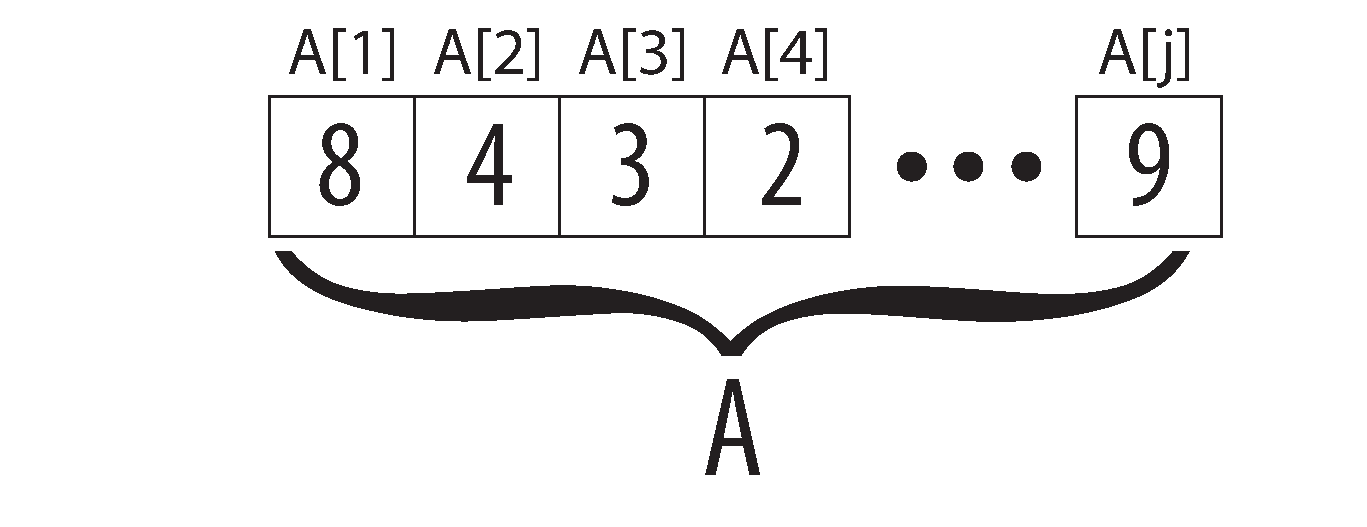
\includegraphics[scale=0.4]{fig/Array.eps}%
		\caption{Illustrasi Array}%
		\label{fig:illustrasiArray}%
	\end{figure}
\end{center}
\begin{Petunjuk}
\label{Ptk:Array}
	\textbf{Penggunaan array}\\
	$A[i] \rightarrow$ Mengakses lokasi ke $i$ dari array yang bernama $A$.\\
	$A[4] \rightarrow$ Mengakses lokasi ke $4$ dari array yang bernama $A$.\\
	$A[i..j] \rightarrow$ Menandakan kumpulan isi array $A$ yang terdiri dari elemen $A[1],\ A[2],\ A[3],\ \ldots,\ A[j]$.\\
	$A[4] = 5 \rightarrow$ Memasukkan nilai 5 ke lokasi ke 4 dari array $A$.\\
	$b = A[4] \rightarrow$ Memasukkan nilai lokasi ke 4 dari array $A$ ke variabel $b$. 
	$A.length \rightarrow$ Menandakan besar/panjang dari array $A$.
	
\marginnote[-4cm]{Catatan : Ilustrasi pada petunjuk ini, hanya menampilkan array 1 dimensi. Seiring dengan meningkatnya pembahasan, akan dikenalkan pada array berdimensi lebih dari satu !}
	
\end{Petunjuk}
	

Petunjuk \ref{Ptk:Array} diatas, beberapa kali menyebutkan istilah \textbf{lokasi}. Pada algoritma ataupun pemrograman, ini lebih dikenal dengan dengan indeks. Walaupun pada gambar \ref{fig:illustrasiArray}, indeks dimulai dari 1(satu), perlu diketahui bahwa pada kebanyakan bahasa pemrograman, termasuk python, indeks pada array selalu dimulai dari 0 dan berakhir pada (panjang data-1). \\

Perhatikan bahwa contoh \ref{Ptk:Array} diatas, sebuah pernyataan tunggal hanya mewakili satu nilai dari sekian banyak data yang ada di dalam array. $A[4]$ misalnya, hanya mengakses indeks ke-4 dari data A. Pertanyaannya adalah bagaimana jika kita memerlukan perhitungan jumlah total dari untuk seluruh data pada array yang berisi bilangan bulat ? Disinilah peran dari struktur perulangan(looping). Agar lebih mengerti mengenai hubungan perulangan dan array, perhatikan contoh berikut ini : 
\pagebreak
 \begin{contoh}
	\textbf{ Jumlah Total Pada Array I}
\begin{listprog}{JumlahTotalArray.py}
\label{lst:JumlahTotalArray}
\begin{lstlisting}[language=Python]
	kumpulanBilangan = [10,20,30,40,50,60,70,80,90,100]
	jumlah = 0
	for i in range(len(kumpulanBilangan)):
		print(kumpulanBilangan[i])
		jumlah += kumpulanBilangan[i]
	print(jumlah)	
\end{lstlisting}
\end{listprog}
\end{contoh}

Contoh \ref{lst:JumlahTotalArray} diatas dibuat sedemikan rupa untuk menunjukkan adanya akses terhadap indeks dari array. Terdapat alternatif lain pengaksesan array melalui looping yang ditunjukkan melalui Contoh \ref{lst:JumlahTotalArray2} berikut : 

 \begin{contoh}
	\textbf{Jumlah Total Pada Isi Array II}
\begin{listprog}{JumlahTotalArray2.py}
\label{lst:JumlahTotalArray2}
\begin{lstlisting}[language=Python]
	kumpulanBilangan = [10,20,30,40,50,60,70,80,90,100]
	jumlah = 0
	for bilangan in kumpulanBilangan:
		print(bilangan)
		jumlah += bilangan
	print(jumlah)	
\end{lstlisting}
\end{listprog}
\end{contoh}

Perhatikan beda contoh \ref{lst:JumlahTotalArray} dan \ref{lst:JumlahTotalArray2}, Pada contoh \ref{lst:JumlahTotalArray} akses bilangan dilakukan dengan akses indeks, sedangkan \ref{lst:JumlahTotalArray2} akses bilangan langsung dilakukan tetapi tanpa akses indeks. Walau tanpa akses indeks, keduanya harus tetap melibatkan struktur perulangan.\\
Sama seperti array bertipe data-lain, Sebuah \textit{String} sebenarnya sudah merupakan array dari karakter. Secara algoritma, Anda dapat mengakses karakter-karakter dari \textit{String}. Perhatikan proses akses array karakter berikut pada algoritma membalikkan kata : 

\begin{contoh}
	\textbf{Membalikkan Kata (\textit{for})}
\begin{listprog}{BalikKata.py}
\label{lst:BalikKata}
\begin{lstlisting}[language=Python]
	kata = ``Mahasiswa``
	
	#start : panjang kata mahasiswa -1 
	#        (indeks terakhir)
	#stop	: berhenti pada saat sudah -1
	#dari start ke stop dengan step : -1
	for i in range(len(kata)-1, -1, -1):
		print(kata[i])
\end{lstlisting}
\end{listprog}
\end{contoh}

\begin{contoh}
	\textbf{Membalikkan Kata (\textit{while})}
\begin{listprog}{BalikKata2.py}
\label{lst:BalikKata2}
\begin{lstlisting}[language=Python]
	kata = ``Mahasiswa``
	indeks = len(kata) - 1
	while(indeks>=0):
		print(kata[indeks])
		indeks -= 1
	\end{lstlisting}
\end{listprog}
\end{contoh}
\end{enumerate}

\FloatBarrier
\subsection{Perulangan Bersarang}
Sebuah perulangan dapat memiliki perulangan di dalamnya dan perulangan yang di dalam tersebut juga dapat juga dapat memiliki perulangan lainnya di dalam. Perulangan yang di dalam tersebut tidaklah harus menggunakan pernyataan yang sama dengan perulangan induknya. Misalnya, boleh saja kita menggunakan pernyataan perulangan \textit{for} di dalam pernyataan perulangan \textit{while} dan juga sebaliknya. Algoritma berikut akan menunjukkan salah satu struktur perulangan bersarang. Ini merupakan salah satu dari kombinasi struktur dasar pada algoritma. \\

Implementasi perulangan lanjut ini akan lebih banyak akan dijelaskan dalam bentuk permasalah - permasalahan pada latihan. Dua permasalahan perulangan bersarang dapat dilihat pada Latihan Menjumlahkan Matriks dan Pencetakan Dengan Baris Kolom.


%\begin{tabbing}
%\textbf{for} $i=n$ \textbf{to} $m$~~~~~~~~~~~~~~~\=\#Mengisi variabel i, dan lakukan perulangan sebanyak (m-n-1)\\
%~~~~~\textbf{for} $j=n$ \textbf{to} $m$~~~~~~~~~~~~~~~\=\#Mengisi variabel j, dan lakukan perulangan sebanyak (m-n-1)\\
%~~~~~statements\\
%~~~~~\textbf{end for}\\
%\textbf{end for}
%\end{tabbing}

\chapter{Latihan : Perulangan}

\begin{pemrograman}
Lakukan perumusan masalah, pembuatan algoritma \& program untuk membuat Urutan dan Deret sebagai berikut : 
\end{pemrograman}

\begin{pemrograman}
Lakukan perumusan masalah, pembuatan algoritma \& program untuk kasus ``Menukarkan Isi Gelas`` jika variabel pada masing - masing gelas memiliki tipe data String !
\end{pemrograman}

\begin{pemrograman}
Lakukan perumusan masalah, pembuatan algoritma \& program untuk kasus ``Menukarkan Isi Gelas`` jika variabel pada masing - masing gelas memiliki tipe data String !
\end{pemrograman}




	
 
